\documentclass[
class = book,
zihao = -4,
font = noto,
paper = a4paper,
openany
]{easybook}

\usepackage{xju}
\newcommand{\ti}{Ti6Al4V}
%笔记
%先模仿,而后进行整改
\begin{document}
	\hypersetup{pdftitle=Ti-6Al-4V 钛合金热处理工艺的研究现状及进展,pdfauthor=田欣洋,pdfsubject={材料科学,金属学,钛合金},pdfkeywords={热处理,固溶,时效,组织},pdfstartview=FitB}
	\maketitle
	\frontmatter*[roman]

	\begin{abstract}
		\ti 合金又名TC4合金,拥有较好的塑韧性、耐热性、成形性、耐蚀性等,在机械、军事、航空航天等领域获得了极为广泛的应用。但TC4合金仍存在硬度较低、摩擦磨损系数高、耐磨性能差、较低的塑韧性和力学性能上的各向异性等缺点,制约了其进一步的应用。
%		初步撰写,模仿《TC4 钛合金热处理工艺的研究现状及进展——孟宪伟袁赵锦秀》
		本文阐述了TC4钛合金的热处理工艺研究现状,并分析了不同热处理制度对Ti6Al4V合金强度的影响,并解析了组织转变的机理,为工程应用提供了有价值的参考,最后提出了TC4钛合金热处理工艺的研究方向。\\

		\keywords{Ti-6Al-4V 钛合金;热处理;显微组织;力学性能;固溶;时效;现状}
	\end{abstract}

	\tableofcontents
	\mainmatter*
	\pagestyle{Xju}
\chapter{前言}
%工业上一般根据$\beta $相稳定元素系数$K_{\beta}$来划分不同类型的钛合金,$K_{\beta}$是指合金中各$\beta $稳定元素与各自的临界浓度的比制之和,即:
%$$
%K_{\beta}=\frac{ C_{1} }{C_{k1}}+\frac{ C_{2} }{C_{k2}}+\frac{ C_{3} }{C_{k3}}+\cdots+\frac{ C_{n} }{C_{kn}}
%$$
%根据 $\beta$ 相稳定系数划分合金类型为:
%
%\begin{table}[htbp]
%	\centering
%	\label{sec:sort}
%	\caption{钛合金类型分类}
%		\begin{tabular}{ccc}
%			\toprule
%			类型&$K_\beta$值&主要合金元素 \\
%			\midrule
%			 $\alpha$ 型& $0 \sim 0.07$&铝、锡、锆\\
%			 近 $\alpha$ 型&$0.07 \sim 0.25$&铝、锡、锆与少量钒、钼、铌\\
%			 $\alpha+\beta$ 型&$0.25 \sim 1.0$&以铝为主、以及其他少量$\beta$ 相稳定元素\\
%			 近 $\beta$ 型&$1.0 \sim 2.8$&少量钒、钼、铌、钽、等\\
%			$\beta$ 型&$ > 2.8 $&大量钒、钼、铌、钽、等\\
%			\bottomrule
%		\end{tabular}
%\end{table}
%其中$\alpha $+$\beta $型钛合金的特点是既有α稳定元素,又有β稳定元素,使α和β同 时 得 到 强 化 。β稳 定 元 素 加 入 量 为 4$ \% $ ~6$ \% $ ,目 的 是 为 了 获 得 足 够 数 量 的β相 ,以 改 善 合 金 的 成 形 塑 性 和 使 合 金 得 到热处理强化的能力,对其进行退火处理,所得到的室温组织为不同比例的$\alpha $和$\beta $相。$\alpha $+$\beta $型钛合金的强度和淬透性随着$\beta $相稳定元素含量增加而提高,其锻造和轧制等加工成型性能优于$\alpha $型、$\beta $型钛合金。从成分上来看,这类钛合金中的合金元素基本上是以铝为主要合金元素,$\beta $稳定化元素为辅助元素。这使得$\alpha $+$\beta $型钛合金组织变动的余地较为灵活,性能变动范围大,可以满足各种应用场合及工况要求\cite{TiandAl}。
%
%我国用TC表示$\alpha $+$\beta $型双相钛合金,最常用的$\alpha $+$\beta $型钛合金包括TC4、TC6、TC12等,其中TC4钛合金(等轴马氏体型两相合金)作为做早被应用的钛合金,该合金以其优越的性能占据了钛工业的大量市场,现在占到 Ti 合金总产量的 50$ \%  $, 占到全部Ti 合金加工件的95$ \% $ 。

TC4钛合金具有较高的抗拉强度和抗疲劳强度、生物相容性好、耐高温、化学性质性质稳定、高硬度和良好的耐腐蚀性、弹性模量低、低密度等优良特性,在航空航天、汽车工业、医疗健康领域等领域得到了广泛应用,是目前应用最广泛的钛合金 。 但其室温塑性较低 , 加工硬化能力较差 , 冷加工成型困难。

近些年关于提升 TC4钛合金室温塑性、强度的相关研究中,国内外研究都取得了许多成果。研究者主要从工艺、组织与性能的关系进行研究,使用的强化手段主要包括添加合金元素、剧烈塑性变形和相变热处理等,对于提高\ti 合金强度、优化加工工艺提供了极具参考价值的建议。但目前关于TC4钛合金热处理工艺研究现状并没有被清晰的表述,尤其是并没有使用计算机技术进行分析,存在笼统、与技术脱节等缺点。针对这些不足,本文将从多个方面对TC4钛合金的研究现状以及未来的发展方向进行科学全面的展望。

\section{优化合金的工艺方法}
钛合金的热处理方式属于共析和有序化转变,在退火和时效过程中存在共析 转变,时效过程中存在有序化转变,现阶段\ti 合金的基本热处理工艺主要有:
\begin{enumerate}
	\item 固溶处理:实施固溶处理工艺,是为了得到等轴稳定的$\alpha $相、马氏体弥散的$ \alpha ^{\prime} $相、亚稳定状态的$\beta $相,等轴的$\alpha $相能够让合金的力学性能得到综合性的提升,马氏体弥散的$ \alpha ^{\prime} $相能够让合金,在强度、硬度上得到提高,塑性、韧性被降低\cite{gurong2002}。
	\item 时效处理:次生的$\alpha $相体积分数在TC4钛合金中,会对屈服强度产生很大的影响。在条件相等的情况之下,时效温度越低组织越小,时效温度高低组织越大。研究人员主要是通过控制参数,来影响对次生$\alpha $相的含量,从而来实现TC4钛合金在力学的性能上得到更好的提升。
	\item 深冷处理:深冷处理是20世纪60年代以来兴起的一种新型冷处理工艺。通过对材料进行-130°C以下的低温处理,可以对金属内部的组织进行改善,并且能够让在热处理之后残留的奥氏体被清除掉。实验研究发现,原始的$\beta $相会在深冷处理的过程当中,逐渐的向$\alpha^{\prime} $相去转变,残余应力在组织中会变少,与此同时网篮状组织的增加,会让TC4钛合金的韧性、强度、塑性,在组织上的性能得到提高。
\end{enumerate}
不同的热处理工艺互相组合可以对合金产生更好的强化效果,现阶段工业上常采用\cite{zhoukaixiangJiyushenlengchulidenanjiagongcailiaoqiexiaotexingyanjiu2022}:淬火+时效;固溶+时效;双重固溶+时效;固溶+双重时效等,其中固溶+时效处理是应用最为广泛的一种热处理工艺组合。
\section{实验用TC4合金的制备与成分}
从制备方式上来看。近些年相关热处理实验中的TC4钛合金大多数是由{多次真空自耗电弧炉熔炼}\cite{renchiqiangGurongshixiaoduiTC4taihejinxianweizuzhihelixuexingnengdeyingxiang2022,ranxingGurongwenduduiTi6Al4VELItaihejinxianweizuzhijixingnengdeyingxiang2021,lilouGurongshixiaoduiTC4hejinzuzhiyujixiexingnengdeyingxiang2014,jingranGurongshixiaoduiTC4hejinzuzhiyuxingnengdeyingxiang2018}而成,其余的是通过粉末冶金\cite{zhanghaoyinGurongShixiaoduiTC4taihejinzuzhihelixuexingnengdeyingxiang2014,xujianGurongshixiaogongyiduiTC4taihejinzuzhijixingnengdeyingxiang2014}的方式来制备TC4,此外还有一小部分用的是热轧合金\cite{LiuWanYingBuTongReChuLiGongYiDuiTi6Al4VTaiHeJinWeiGuanJieGouHeLiXueXingNengYingXiangYingWen2017}、电子束选区熔化合金\cite{leijunleDianzishuxuanquronghuachengxingTC4hejinxianweizuzhiyuxingnengdeyanjiujinzhan2022}、商用棒状TC4合金\cite{LuYuanYuanShiXiaoChuLiDuiTC4TaiHeJinWeiGuanZuZhiHeLiXueXingNengDeYingXiang2019}等。其中真空自耗电弧炉熔炼得到的合金强度普遍较高,而粉末冶金法虽然工艺复杂,但其得到的组织晶粒细小、成分偏析少、机加工量减小,是TC4合金制备的新趋势。

从化学成分上来看。标准的TC4钛合金成分有国家标准:
\begin{table}[htbp]
	\centering
	\label{sec:mytc4chem}
	\caption{TC4合金化学成分的国家标准}
	\begin{tabular}{cccccccc}
		\toprule
		元素($ \% $) & Al & V &Fe &C& O& N &H \\ \midrule
		标准要求 &$ 5.5\sim 6.75 $ & $ 3.5\sim 4.5 $&$ \le 0.30 $ & $ \le 0.05 $&$ \le 0.20 $&$ \le 0.03$ &$ \le 0.015 $  \\ \bottomrule
	\end{tabular}
\end{table}
%开始废话填充模式。2023-1-9-13:05


本文统计了近年\ti 钛合金热处理研究方面的近十多篇文献,发现不同实验者在试验中用到的合金成分都有所差异,如\ref{sec:mytc4ave}所示。其中Al元素的含量差异较大,从$ 5.65\% $到$ 6.4\% $不等,v元素的含量差异较小,都在$ 3.97 \%$到$ 4.25\% $范围之间,其余的非主要的杂质元素成分如Fe、C、N、O等的含量也有不同,总的来讲含量都在国标的范围之内。
\begin{table}[htbp]
	\centering
	\caption{不同实验者所用的TC4合金元素统计}
	\label{sec:mytc4ave}
	\begin{tabular}{ccccccccc}
		\toprule
元素($ \% $)& Ti  & Al & V &Fe &C& N& O &H \\ \midrule
平均值 & 89.455 & 6.118 & 4.086 & 0.102 & 0.028 & 0.039 & 0.164 & 0.007 \\
方差 & 0.147 & 0.253 & 0.104 & 0.074 & 0.019 & 0.078 & 0.060 & 0.015 \\
标准差 & 0.022 & 0.066 & 0.011 & 0.006 & 0.000 & 0.006 & 0.004 & 0.000 \\
最大值 & 89.73 & 6.4 & 4.25 & 0.3 & 0.08 & 0.2 & 0.27 & 0.04 \\
最小值 & 89.344 & 5.65 & 3.97 & 0.03 & 0.009 & 0.001 & 0.09 & 0 \\
极差 & 0.386 & 0.75 & 0.28 & 0.27 & 0.071 & 0.199 & 0.18 & 0.04 \\
		\bottomrule
	\end{tabular}
\end{table}




\chapter{固溶处理}
固溶处理作为TC4钛合金的主要强化手段,能够显著改善合金的力学性能、机械加工性能以及耐热性能等,应用极为广泛。

就固溶处理的工艺参数而言,温度的选择至关重要。如果固溶温度过低,则相变无法充分进行,难以获得完全的$\beta$相,导致性能提高有限;反之,如果固熔溶温度过高,会引起$ \beta $相的粗化,导致材料强度降低。只有在最佳的固溶温度范围,合金才能获得最佳的微观组织:板条状a相之间分布着细小的b相,此时的性能最好。

下面本文就从\textbf{固溶温度的选择}、\textbf{固溶处理对组织性能的影响}两个方面来介绍\ti 合金的固溶处理工艺。

\section{固溶处理得到的组织与性能}
对于固溶处理过程,常见的组织为典型双态组织:球状的初生$ \alpha_p $相、板条状$ \alpha $相、细小的$ \beta $相转变组织以及部分粗大的$ \beta $相转变组织\cite{zhanghaoyinGurongShixiaoduiTC4taihejinzuzhihelixuexingnengdeyingxiang2014},固溶温度对Ti6Al4V 钛合金显微组织形貌的影响主要在于 初生$ \alpha_p $相含量、片层$ \alpha $相厚度以及$\beta$晶粒尺寸,其中粗大的初生$ \alpha_p $相组织,对性能的影响较大,是不利因素;片层状$ \alpha $相是有利组织,可以很好地提高组织的的强度\cite{ranxingGurongwenduduiTi6Al4VELItaihejinxianweizuzhijixingnengdeyingxiang2021}。取向越无序、性能越差,最佳组织为\textbf{板条状α相组织之间分布着较为细小的$\beta$相转变组织}、\textbf{越粗大、取向越不规律},则性能越差。
\begin{figure}[h!]
	\centering
	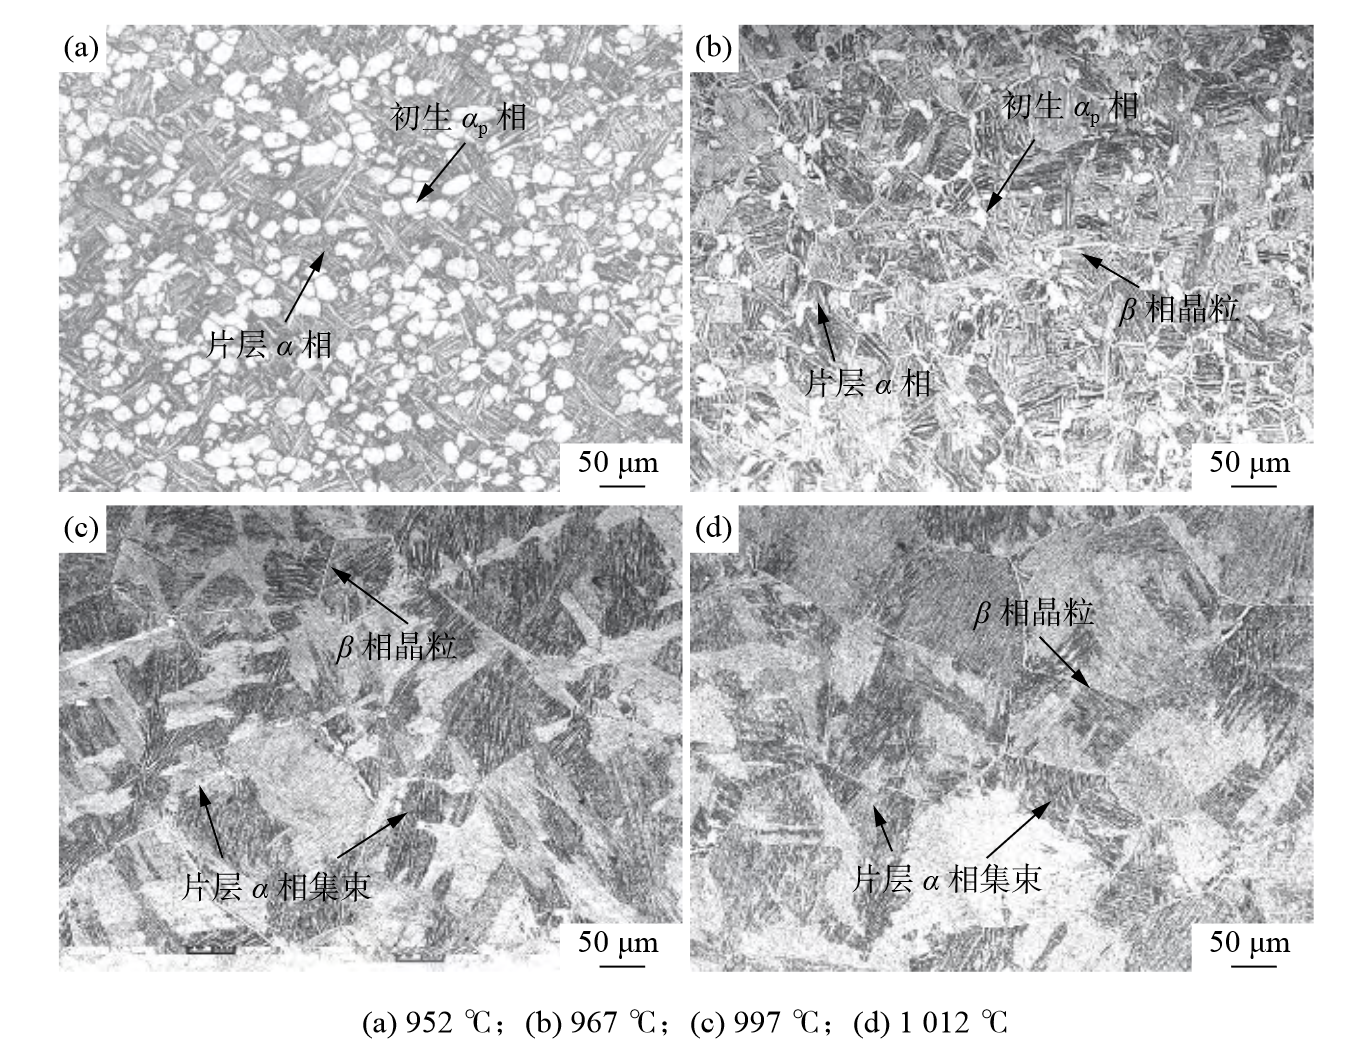
\includegraphics[width=0.7\linewidth]{金相_丙}
	\caption{不同固溶温度下TC4合金的显微组织}
	\label{fig:}
\end{figure}


总的来讲,固溶的作用是将粗大的双态组织均匀化,减小不同相之间的取向差异,从性能上来看,得到恰当成分的b相最有利于强度。

%\chapter{热处理工艺对力学性能的影响}
\section{相变点的计算与固溶温度的选择}
$\beta$转变温度是钛合金的重要参数之一,它是制定钛合金的热机械工艺和热处理工艺的重要依据,相变过程如\ref{sec:Tc4betachange}所示。郭凯\cite{guokaiTC4taihejinrechuligongyideyanjiuxianzhuangjijinzhan2021}等人表示:当固溶温度高于 $\beta$ 相变时的温度时,合金的强度伴随温度的增加而下降,而且残余应力也开始大幅度的降低;当固溶温度低于 $\beta$ 相变时的温度时,合金的强度伴随温度的增加而增加,残余应力也略微提高。但是徐戊矫、谭玉全\cite{xujianGurongshixiaogongyiduiTC4taihejinzuzhijixingnengdeyingxiang2014}却表明:在相变点以下,随着退火温度的升高,材料的 强度、塑性和冲击韧性呈降低趋势。之所以会出现这种完全相反的结论,很可能是研究者对于相变点的具体值定义不清晰导致的,可见相变点的确定在固溶处理过程中是非常关键的。

近年来,确定$ \beta $相变点的常见计算方法\cite{zhuhongTaihejinaVxiangbiandiandejizhongceshifangfatantao2013}主要有:连续升温金相法、X 射线衍射法、电阻法、等热膨胀法、元素含量法和神经网络模型预测预测法\cite{renchiqiangGurongshixiaoduiTC4taihejinxianweizuzhihelixuexingnengdeyingxiang2022}等。
\begin{table}[htbp]
	\centering
	\caption{\ti 合金$ \alpha+\beta \to \beta $转变时发生的相变及存在的相}
	\label{sec:Tc4betachange}
\begin{tabular}{ccc}
	\toprule 室温相 & 相变过程 & 高温相 \\
	\midrule$\alpha-\mathrm{Ti}$ & $\alpha-T i \rightarrow \beta-T i$ & $\beta-\mathrm{Ti}$ \\
	$\alpha-\mathrm{Ti}-\mathrm{Al}$ & $\alpha-\mathrm{Ti}-\mathrm{Al} \rightarrow \beta-\mathrm{Ti}+\beta-\mathrm{Ti}-\mathrm{Al}$ & $\beta-\mathrm{Ti}, \beta-\mathrm{Ti}-\mathrm{Al}$ \\
	$\beta- \mathrm{Ti}-\mathrm{V}$ & $\beta-\mathrm{Ti}-\mathrm{V} \rightarrow \beta^{-} \mathrm{Ti}-\mathrm{V}$ & $\beta-\mathrm{Ti}-\mathrm{V}$ \\
	\bottomrule
\end{tabular}
\end{table}

\begin{enumerate}
	\item 元素含量法:根据合金中各元素对相变温度的影响来对相变点进行推算,通过\ref{sec:chem4ti}所示\cite{ananyaLocationBasedIntelligent2011}的因素,利用经验公式\ref{jingyan}来计算。
	\begin{equation}
		\begin{aligned}
			T_{\alpha+\beta / \beta \text { 相变点 }}=&872{ }^{\circ} \mathrm{C}-7.7[\mathrm{Mo}]-5.5[\mathrm{V}]-13.8[\mathrm{W}]- 10.6[\mathrm{Nb}]-15.6[\mathrm{Ta}]\\
			&-2.8[\mathrm{Cr}]-5.6[\mathrm{Cu}] +4.4[\mathrm{Ni}]+3.3[\mathrm{Co}]+4.4[\mathrm{Mn}]+23.4[\mathrm{Al}] \\
			& -4.3[\mathrm{Zr}]-8.4[\mathrm{Fe}]+32.1[\mathrm{Si}]
		\end{aligned}
		\label{jingyan}
	\end{equation}
	\item 膨胀法:根据金属在加热过程中用发生相变时新相与母相的膨胀系数不同或比容 发生变化而确定相变点。
	\item 金相法:在钛合金理论相变温度附近每隔5°C或10°C热处理1个样品,在金相显微镜下观察到无剩余$\alpha$相的试样,将比该试样热处理温度低5°C的温度计为钛合金的$\alpha+\beta/\beta$相转变温度。
\end{enumerate}
\begin{table}[htbp]
	\centering
	\caption{部分元素含量对钛合金相变点的影响}
	\label{sec:chem4ti}
\begin{tabular}{cccc}
	\hline 元素名称 & 元素含量 $(\mathrm{Wt} \%)$ & 差值&累积值 \\
	\hline $\mathrm{Al}$ & $2.0 \sim 7.0$ & $23.0^{\circ} \mathrm{C} / 1.0 \%$ & $+143.0^{\circ} \mathrm{C}$ \\
	$\mathrm{V}$ & $0 \sim 10.0$ & $-14.0^{\circ} \mathrm{C} / 1.0 \%$ & $-140.0^{\circ} \mathrm{C}$ \\
	$\mathrm{Fe}$ & $0 \sim 15.0$ & $-16.5^{\circ} \mathrm{C} / 1.0 \%$ & \\
	$\mathrm{Si}$ & $0 \sim 0.45$ & $-1.0^{\circ} \mathrm{C} / 0.1 \%$ & $ -4.5^{\circ} \mathrm{C} $\\
	$\mathrm{C}$ & $0 \sim 0.15$ & $+2.0^{\circ} \mathrm{C} / 0.01 \%$ &$ +30.0^{\circ} \mathrm{C} $\\
	$\mathrm{O}$ & $0 \sim 1.0$ & $+2.0^{\circ} \mathrm{C} / 0.01 \%$& \\
	$\mathrm{~N}$ & $0 \sim 0.5$ & $+5.5^{\circ} \mathrm{C} / 0.01 \%$& \\
	$\mathrm{H}$ & $0 \sim 0.50$ & $-5.5^{\circ} \mathrm{C} / 0.01 \%$ &\\
	\hline
\end{tabular}
\end{table}



关于$\beta$转变温度的具体值,目前广泛认同的是位于975℃附近,但是由于不同试样的合金元素的种类与含量的差异,尤其是局部化学成分的差异,使得不同研究人员实际测得的相变点温度有所差异\cite{wangtaoTC4hejinxiangbianwendujiancezhongjieguobuyizhiyuanyinfenxi2013}。

姚德人等\cite{yaoderenTc4taihejinxiangbiandiandeceding1975}表明相变温度为975℃到980℃之间,此时的合金拥有最低的硬度,当温度略大时会发生$\beta$晶粒的显著长大;相变点以下50℃以内水淬,可以得到不同数量的初生$ \alpha $和马氏体$ \alpha^{\prime} $,而后再进行低温退火时,马氏体$ \alpha^{\prime} $又会转变为稳定的次生$ \alpha$和$ \beta $,可以得到较好的综合性能\footnote{\color{red}此文章写于1975年,但是仍然非常有参考价值}。刘伟东等人\cite{liuweidongTC4hejinVzhuanbianwendudejinxiangfacedingyulilunjisuan2014}通过连续升温金相法,使用EET\footnote{Empirical Electron Theory of solids and molecules“固体与分子经验电子理论”(简称余氏理论)}模型建模测得了\ti 合金的相变温度为974.58℃;孙宇、曾卫东等人\cite{sunyuYingyongrengongshenjingwangluoyanjiuhuaxueyuansuduitaihejinxiangbiandiandeyingxiang2010}通过人工神经网络ANN技术,运用反向传播算法,建立了三层神经网路-钛合金相变预测模型,最终预测得到在绝对误差为9.8℃的情况下,TC4的相变点为994.8℃。

可见通过不同手段测得的相变温度差异是比较大的,未来的主要研究方向应该是,消除不同合金中局部化学成分的差异的影响,利用不同测量手段的优缺点,结合多种方式与计算机技术,最终建立起一个适用性更强的计算模型,以方便确定不同元素含量的TC4合金的相变点。
%通过合金元素的含量进行计算\footnote{《基于二元相图精确计算钛合金α+β/β相变点》}:
%\begin{figure}[h!]
%	\centering
%	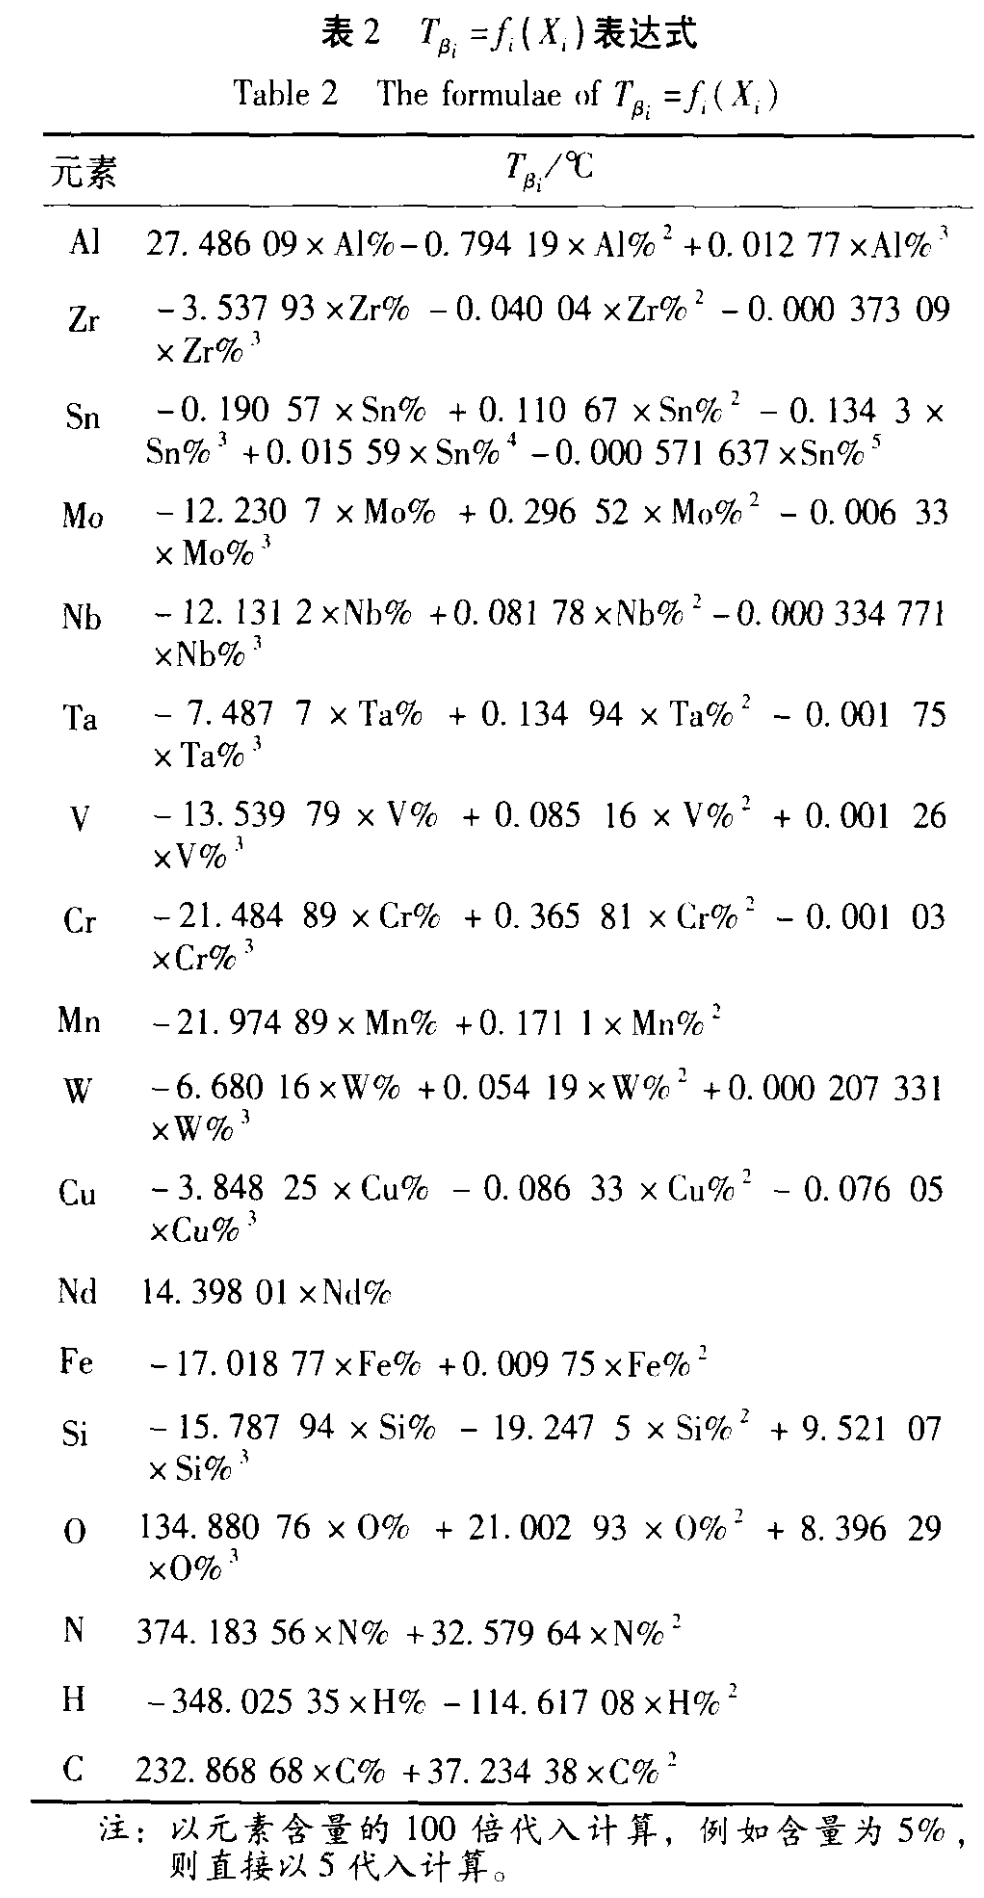
\includegraphics[width=0.8\linewidth]{相变点计算}
%	\caption{相变点计算}
%	\label{fig:keypoint}
%\end{figure}
\section{冷却速度的影响}
固溶处理过程中,常见的冷却方式有炉冷、水冷、油冷、空冷等,而不同的冷却速率会产生不同的$ \alpha  $、$ \alpha  ^{\prime}$、$ \alpha  ^{\prime\prime}$、$ \beta$相微观组织\cite{malinovModellingCorrelationProcessing2001}。Ahmed T, Rack H J等人通过顶端淬火\footnote{顶端淬火试验,又称Jominy试验。是一种测定淬透性的简便方法。做法是用标准试样经适当奥氏体化后进行顶端淬火。顶端淬火时冷却速度由淬火端沿试棒逐渐减小,组织和硬度随之相应地变化,由此得到的硬度变化曲线称为淬透性曲线或Jominy曲线。}的方式研究\cite{ahmedPhaseTransformationsCooling1998}了不同冷却速度下的\ti 合金组织,发现:只有当冷却速度较大于410°$C  s^{- 1} $时,才会发生完全的马氏体转变;当冷却速度小于此值时,会在$ \beta $相晶界出析出二次块状$\alpha  $相与$ \alpha^{\prime} $相的混合组织;当冷速达到小于20°C °$C  s^{- 1} $时,这种转变会逐渐被典型的魏氏体组织转变取代,结论如\ref{fig:tc41050c3}所示:
\begin{figure}[h!]
	\centering
	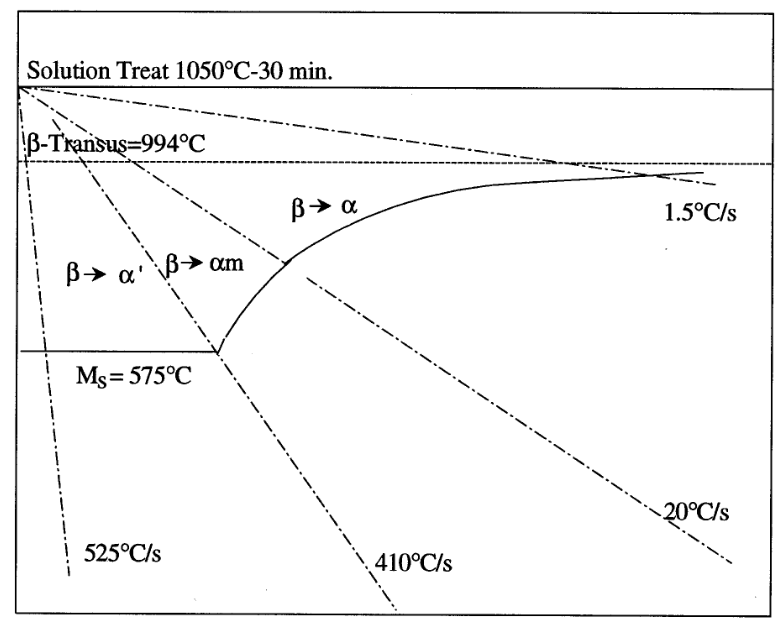
\includegraphics[width=0.7\linewidth]{TC4在1050℃连续3冷分钟却示意图}
	\caption{TC4在1050℃连续3冷分钟却示意图}
	\label{fig:tc41050c3}
\end{figure}


甘章华、梁宇等人研究发现\cite{ganzhanghuaRechuligongyiduiTC4taihejinzuzhijiyingdudeyingxiang2014}TC4钛合金在1020℃进行保温后, 炉冷组织为排列紧密且粗大的$\alpha $相, 空冷组织为粗短的$\alpha $相, 油冷组织为$\alpha $相和少量针状马氏体$\alpha^{\prime}$相, 水冷组织为细针状$\alpha^{\prime}$相,如\ref{fig:tc4970c}所示。随保温温度升高至1100℃、1200℃, 炉冷和空冷组织变粗大的,而水冷时均得到马氏体组织,如\ref{fig:tc41100c}所示。徐戊矫、谭玉全等人研究\cite{xuwujiaoTuihuowenduhelengquesushuaiduiTC4taihejinzuzhihexingnengdeyingxiang2016}发现:冷却速度越大,得到的马氏体$ \alpha^{\prime} $越多,材料内部的位错越多,导致材料的冲击韧性越差,因而使用炉冷的方式可以很好地提高合金的塑韧性。 未来的研究方向应该是分析冷却速度对于马氏体组织、片层状$ \alpha $相组织形成的影响,以得到塑韧性、强硬度都比较好的\ti 合金。
\begin{figure}[htbp]
	\centering
	\begin{minipage}[t]{0.48\textwidth}
	\centering
	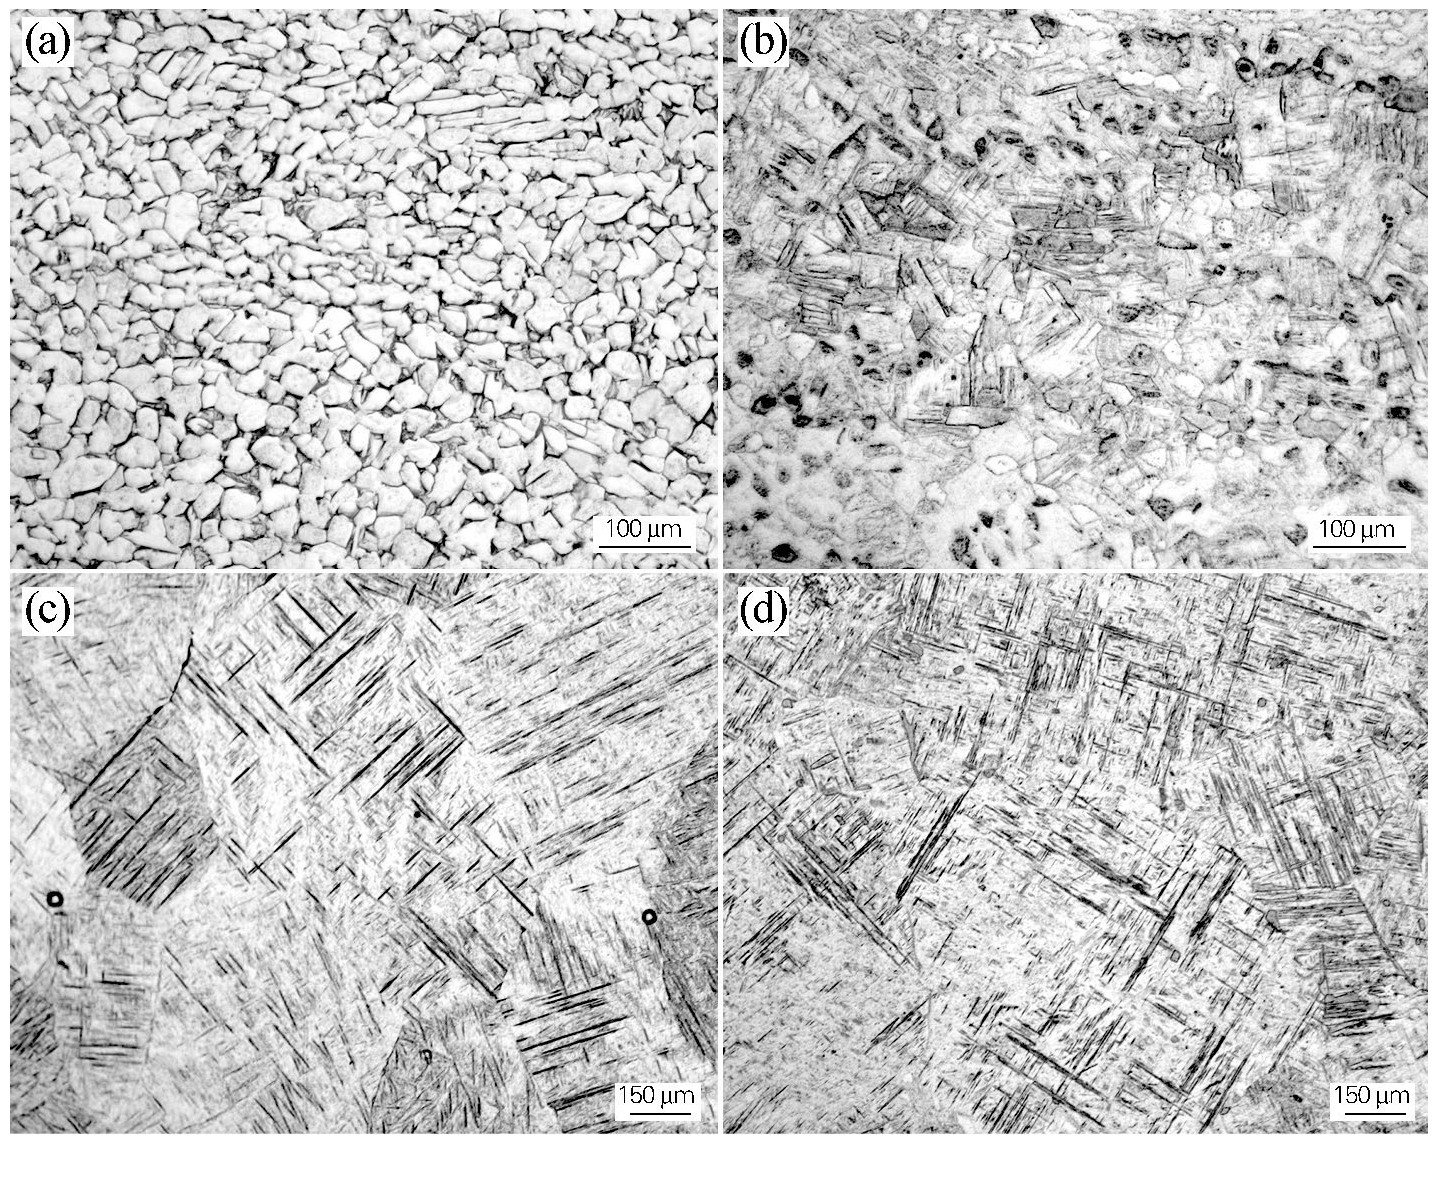
\includegraphics[width=0.7\linewidth]{TC4合金970℃加热后不同冷却方式下的显微组织}
\caption{TC4合金970℃加热后不同冷却方式下的显微组织\cite{ganzhanghuaRechuligongyiduiTC4taihejinzuzhijiyingdudeyingxiang2014}(a) 炉冷; (b) 空冷; (c) 油冷; (d) 水冷}
\label{fig:tc4970c}
	\end{minipage}
	\begin{minipage}[t]{0.48\textwidth}
	\centering
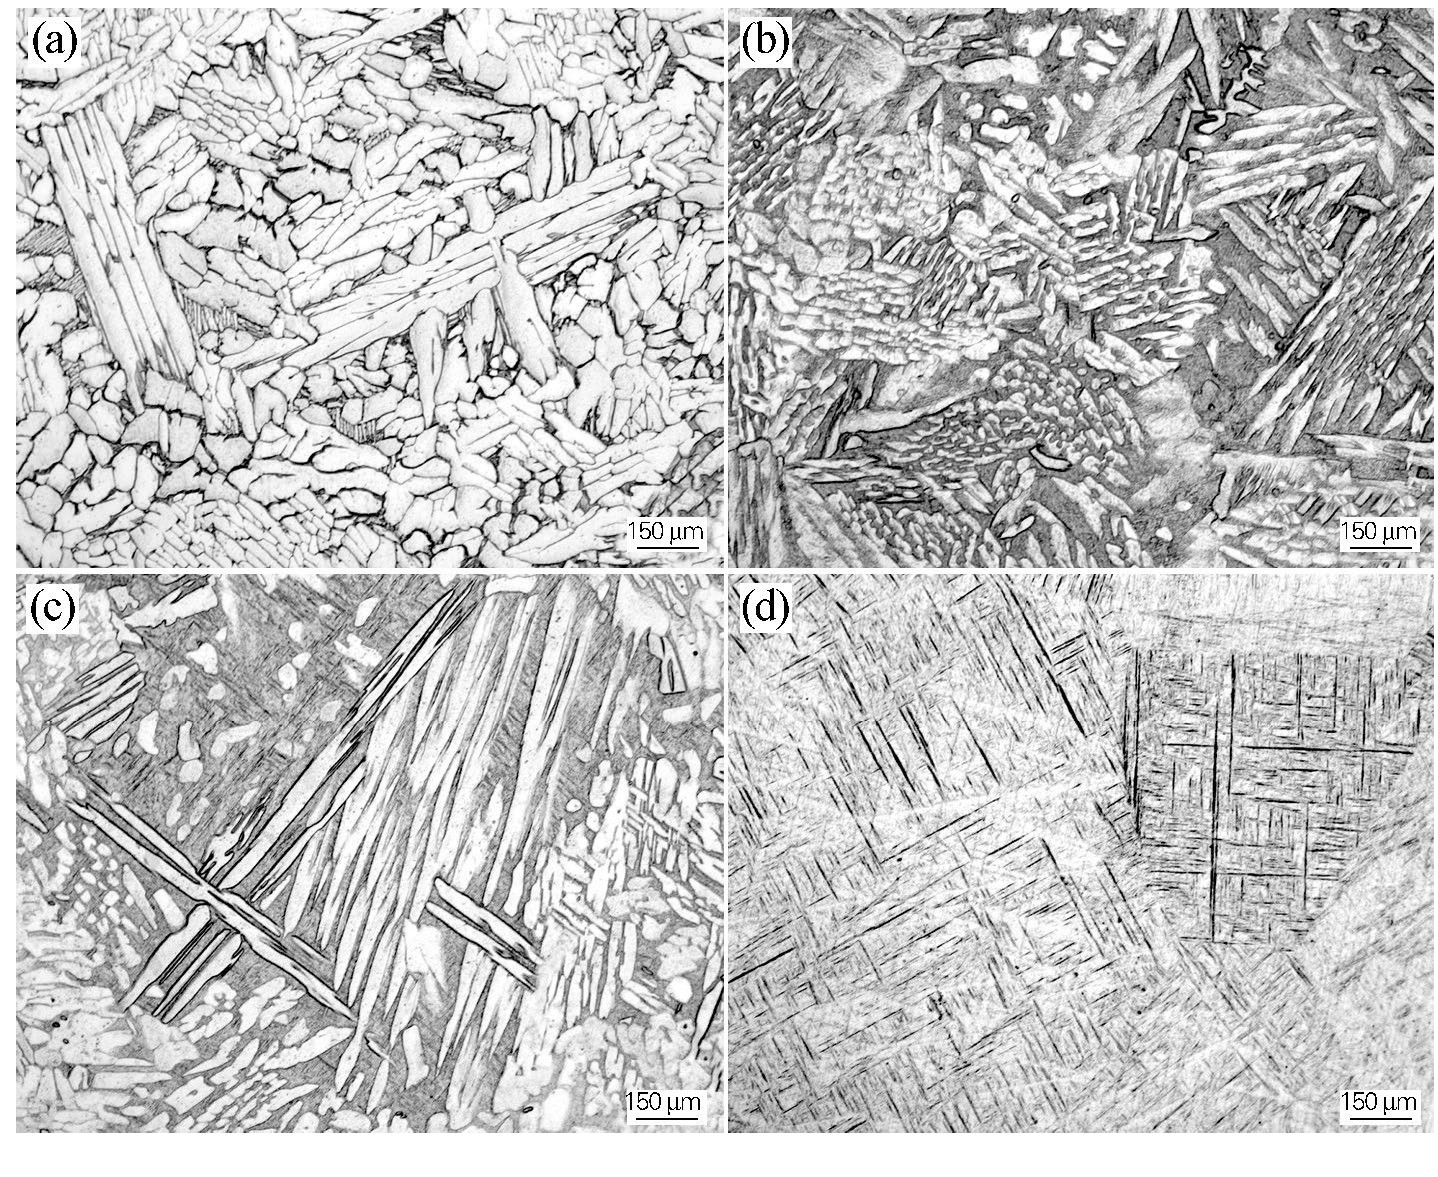
\includegraphics[width=0.7\linewidth]{TC4合金1100℃加热后不同冷却方式下的显微组织}
\caption{TC4合金1100℃加热后不同冷却方式下的显微组织(a) 炉冷; (b) 空冷; (c) 油冷; (d) 水冷}
\label{fig:tc41100c}
	\end{minipage}
\end{figure}

\chapter{时效处理}
时效是在较低温度下对淬火组织保温一段时间后进行空冷的热处理工艺,可以显著提高合金的强度。对于\ti 合金而言,一般整个过程的温度都在 650°C以下。发生的相变有 $ \alpha  ^{\prime}\to \beta+\alpha$、$ \alpha  ^{\prime\prime}\to\beta+\alpha$和 $\omega\to \alpha+\beta$
\section{时效处理得到的组织与性能}

对于时效处理过程,出现的组织为$ \alpha  ^{\prime}$相,$ \alpha  ^{\prime}$相脱溶出来的等轴$ \alpha$相与$ \beta $相、变粗大的$ \alpha $相与$ \beta $相\footnote{固溶后钛合金中马氏体仍保持$ \alpha $相软而韧的性能,在随后进行的时效强化使得马氏体分解,获 得 弥 散 的轴$ \alpha+\beta $组织,从而进一步提高其抗拉强度。 随 着 时 效 温度的升高,伸长率逐 渐 上 升,但是抗拉强度则呈下降 趋势。}。\cite{zhanghaoyinGurongShixiaoduiTC4taihejinzuzhihelixuexingnengdeyingxiang2014}时效的作用就是将固溶后得到的亚稳定组织低温热处理, 促使亚稳定组织 $\beta$ 相、$ \alpha  ^{\prime}$相及 $ \alpha  ^{\prime\prime}$相转变为细小、稳定 的等轴组织与片层组织以起到弥散强化作用。


经过调研发现,在大多数实验中当固溶温度选取在低于$ \beta $相变温度50度左右时,得到的性能最好。

\section{时效温度的确定与二次β相的分解}


\section{时效时间}


\chapter{固溶时效对于强度的影响}

\section{现阶段研究对于合金性能的强化效果}
从强度上来看,大多数试样的抗拉强度在850Mpa以上,屈服强度在830Mpa以上,基本满足国家标准\ref{sec:mytc4machin}。在调研过程中发现,经过固溶、时效等热处理方式处理过后,试样的抗拉强度与屈服强度增加了200Mpa左右,分别达到了900Mpa与1200Mpa之间。其中,最高的强度是鲁媛媛等\cite{LuYuanYuanShiXiaoChuLiDuiTC4TaiHeJinWeiGuanZuZhiHeLiXueXingNengDeYingXiang2019}在970℃$ \beta $相变点附近进行固溶处理后,再通过550℃/300min(AC)方式下得到的组织,其抗拉强度$ \sigma_m $达到了1218Mpa,屈服强度\footnote{标准术语为“塑性延伸强度”,当塑性延伸率为$0.2\%  $时即为屈服强度}为$ \sigma_{0.2} $为1109Mpa,可见热处理对于组织的优化还是很可观的。
\begin{table}[htbp]
	\centering
	\caption{TC4合金力学性能的国家标准}
	\label{sec:mytc4machin}
	\begin{tabular}{cccc}
		\toprule
		力学性能& 抗拉强度$Mpa  $& 屈服强度$ Mpa $&断后伸长率$ \% $\\ \midrule
		标准值 &$ \ge 895 $&$ \ge 830 $&$ \ge 10 $ \\ \bottomrule
	\end{tabular}
\end{table}


\begin{table}[htbp]
	\centering
	\caption{不同实验所得的TC4强度统计}
	\label{sec:mytcstrengthave}
	\begin{tabular}{cccc}
		\toprule
		类型& $ \sigma_{0.2} $屈服强度/Mpa  &$ \sigma_m $抗拉强度/Mpa &延伸率$ \delta \% $ \\ \midrule
		平均值 & 953.541& 1001.874&12.160 \\
		方差 &97.116& 105.897& 4.077 \\
		标准差 &9656.014&11438.403&16.952 \\
		最大值 &  1110 & 1218 & 19 \\
		最小值&700 & 790 & 3.78 \\
		极差&410 & 428 & 15.22 \\
		\bottomrule
	\end{tabular}
\end{table}




在不同固溶温度的处理下,可以得到不同的组织,进而呈现出不同的力学性能。如\ref{fig:固溶温度与强度}所示,通过分析可得:研究者集中在900到1000℃之间进行研究,且在温度达到960℃附近的时候,合金拥有相对较大的屈服强度与抗拉强度。

\begin{figure}[h!]
	\centering
	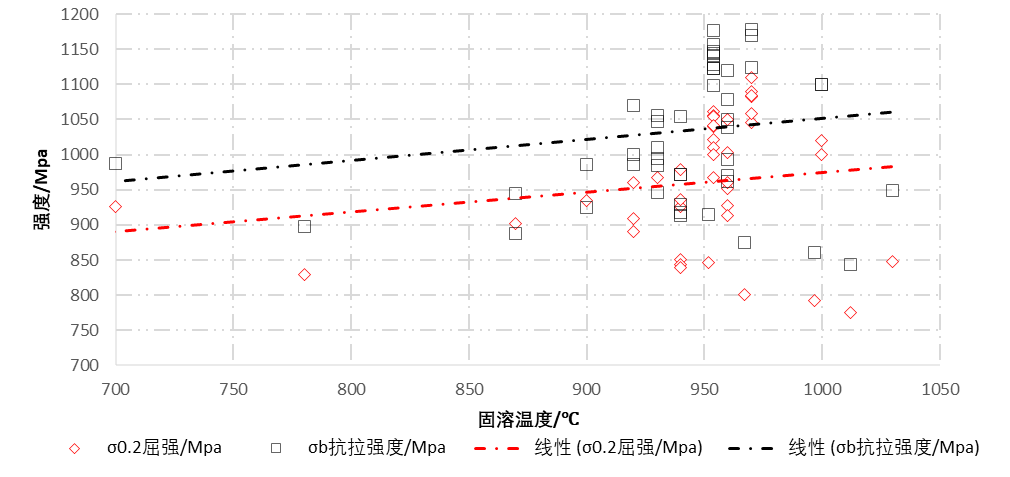
\includegraphics[width=0.7\linewidth]{固溶温度与强度}
	\caption{固溶温度与强度}
	\label{fig:固溶温度与强度}
\end{figure}

如\ref{fig:时效温度与抗拉屈服强度}所示,通过分析可得,研究者集中在500℃与725℃附近,且前者温度附近时效处理得到的合金强度较大。
\begin{figure}[h!]
	\centering
	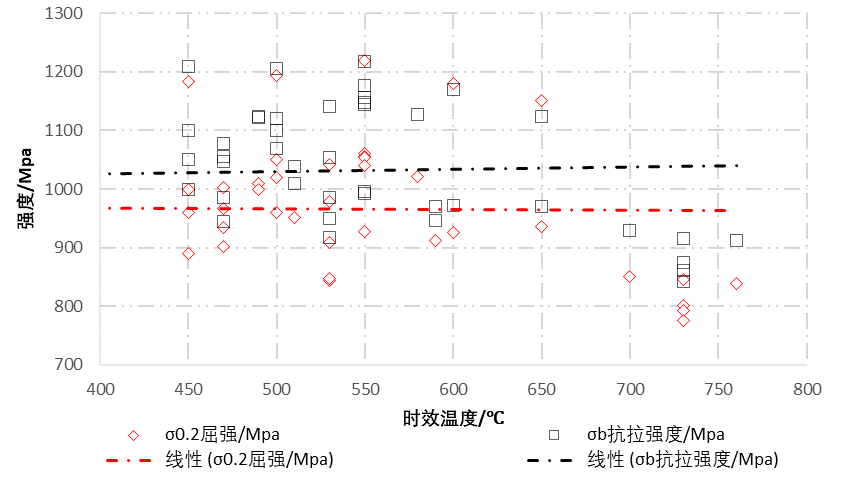
\includegraphics[width=0.7\linewidth]{时效温度与强度}
	\caption{时效温度与抗拉屈服强度}
	\label{fig:时效温度与抗拉屈服强度}
\end{figure}

\section{研究现状与展望}
 刘婉颖、林元华等人通过实验发现:在960 ℃/1 h + WQ进行固溶处理和500 ℃/4 h + AC下进行时效处理得到的\ti 具有最佳的力学性能\cite{LiuWanYingBuTongReChuLiGongYiDuiTi6Al4VTaiHeJinWeiGuanJieGouHeLiXueXingNengYingXiangYingWen2017};陈冠宇通过实验表明,在850℃进行退火处理时,在600℃进行时效处理可以使合金得到更好的耐腐蚀性能\cite{1200};李宸宇证明\ti 合金在900℃空冷固溶两小时在530℃时效四小时后具有更好的强硬度,而且固溶后冷速越快,合金的强硬度越高、塑韧性越差\cite{900}。%第46页
\chapter{结论}




	\backmatter
	\listoffigures
	\listoftables
	\clearpage
	\phantomsection
	\addcontentsline{toc}{chapter}{参考文献}
	\bibliography{modern}
\end{document}


